\section{Conservation of Total Budget and Infinite Decomposition of the Great Circle}

\begin{figure}[ht]
\centering
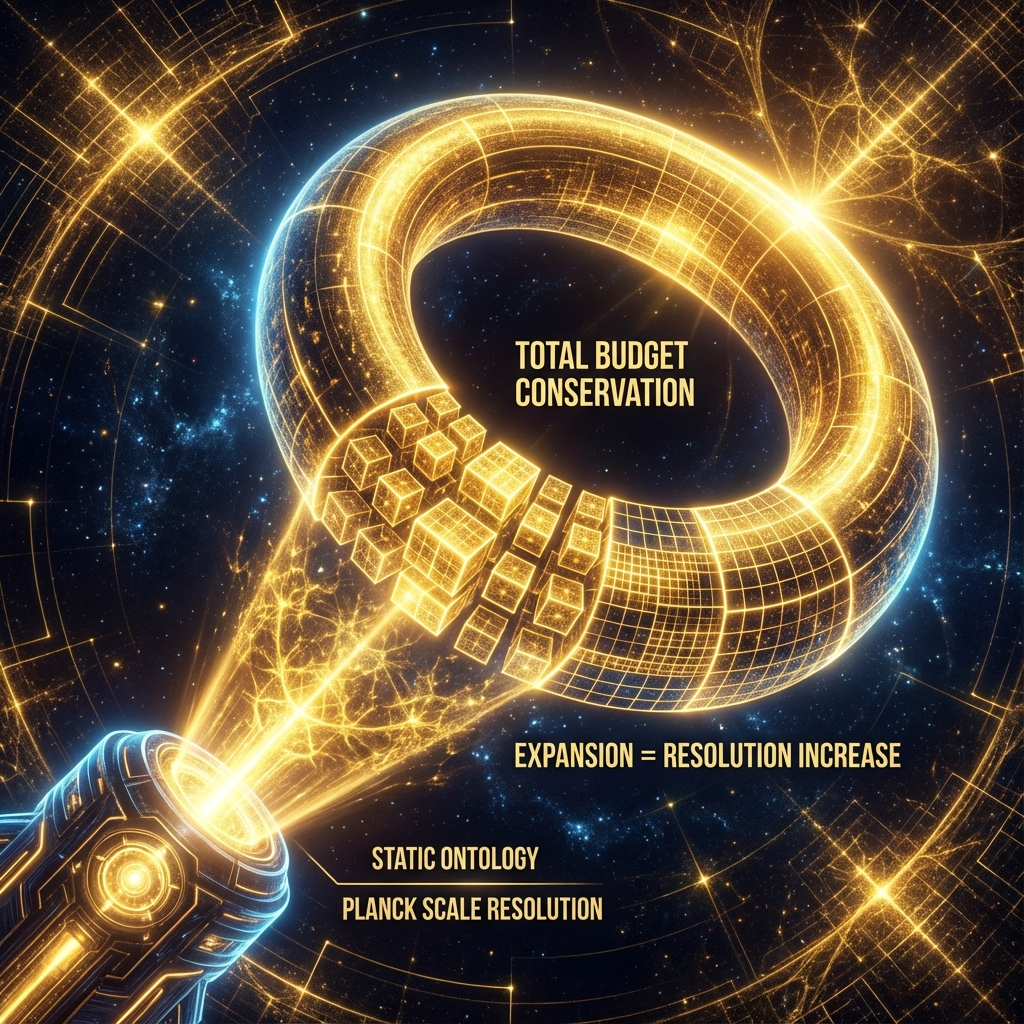
\includegraphics[width=0.8\textwidth]{assets/chapter05-04-total-budget-conservation.png}
\caption{Total Budget Conservation}
\end{figure}

In the previous section, we derived the entropic nature of gravity through holographic thermodynamics and revealed that spacetime curvature is a manifestation of computational lag. However, the exponential growth of light speed $c(\tau)$ and the continuous proliferation of spacetime grids in Omega Theory seem to imply that the universe's total energy is increasing infinitely over time. This directly challenges the cornerstone of physics---the conservation laws guaranteed by Noether's Theorem. If spacetime lacks time translation invariance, energy conservation appears to fail.

This section will resolve this fundamental contradiction. We will introduce the concept of \textbf{``Total Budget Conservation''}, proving that cosmic evolution is not the ``creation from nothing'' of physical entities, but rather the \textbf{infinite Fibonacci decomposition} of a \textbf{Great Circle} in Hilbert space. The total quantity of the universe never changes; only the holographic resolution changes.

\subsection{Normalization Axiom: The Total Budget of Existence}

In standard cosmology ($\Lambda$-CDM), as space expands, dark energy density remains constant, causing the universe's total energy to increase linearly with volume. This is usually explained as ambiguity in the definition of energy in general relativity. But in the axiomatic system of Omega Theory, we must adhere to stricter mathematical constraints.

According to the \textbf{Omega Axiom} proposed in Chapter 0, the universe is a single static vector $|\Omega\rangle$ in Hilbert space $\mathcal{H}$. The probabilistic interpretation of quantum mechanics requires this vector to be \textbf{normalized}:
\[\langle \Omega(\tau) | \Omega(\tau) \rangle \equiv 1\]

We define this dimensionless ``1'' as the universe's \textbf{``Ontological Total Budget'' ($B_{total}$)}.

\textbf{Definition 5.2 (Budget Conservation Axiom)}:
Regardless of how many particles, galaxies, or bits emerge within the universe, and regardless of how intrinsic time $\tau$ evolves, the system's total measure of information is strictly conserved. Physical evolution $\hat{U}(\tau)$ is a pure rotation (unitary transformation) acting on the unit sphere; it neither creates nor destroys ``existence'' itself.

This means that the ``cosmic expansion'' and ``energy explosion'' we observe are essentially a \textbf{Perspective Illusion}. They arise from the observer's own scale \textbf{relative contraction}.

\subsection{Fibonacci Decomposition Topology}

To visualize this abstract process, we map the phase structure of Hilbert space to the \textbf{unit circle $S^1$} (the great circle) in the complex plane.

Cosmic evolution can be geometrized as \textbf{``Golden Angle Slicing''} performed on this great circle.
Let the initial moment be $\tau=0$, where the great circle is an undivided whole (full frequency band).
As the golden unitary operator $\hat{U}_g$ acts, each intrinsic time step $\tau \to \tau+1$ corresponds to cutting the circle once, generating a new basis vector. The cutting angle strictly follows the golden angle $\theta_g$:
\[\theta_g = 2\pi \left( 1 - \frac{1}{\phi} \right) \approx 137.50776^\circ\]

Due to the irrationality of $\phi$, according to Weyl's equidistribution theorem (see Section 1.1), these cut points will never coincide.

\begin{itemize}
\item \textbf{When $\tau$ is small}: The circle is only divided into a few rough arcs. This corresponds to the early universe, where physical laws are vague and particle types are scarce.
\item \textbf{When $\tau \to \infty$}: The circle is divided into infinitely dense segments, but the sum of lengths of these infinitely many arcs always equals $2\pi$.
\end{itemize}

\begin{figure}[ht]
\centering
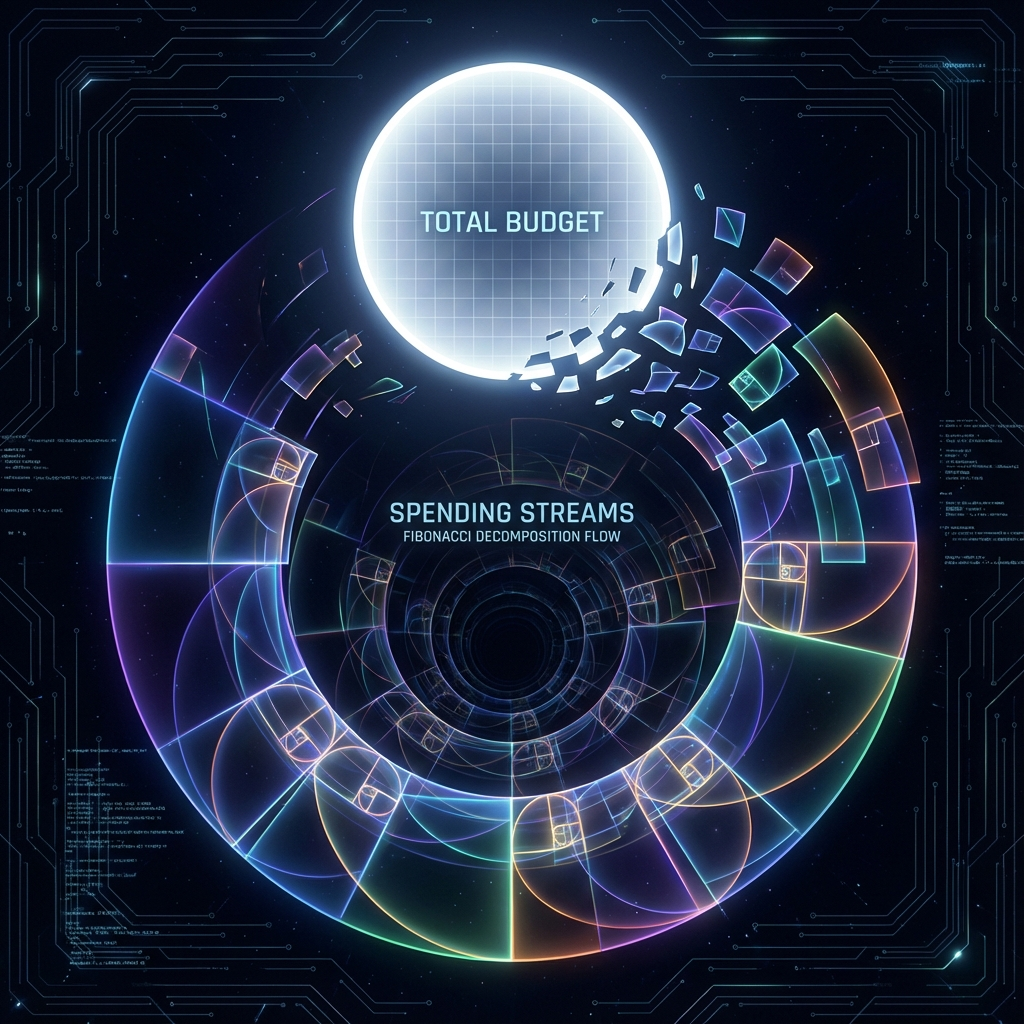
\includegraphics[width=0.8\textwidth]{assets/chapter05-04-total-budget-decomposition.png}
\caption{Total Budget Decomposition}
\end{figure}

\textbf{Theorem 5.4 (Decomposition Equivalence Theorem)}:
The Fibonacci spiral growth of the universe is topologically equivalent to the \textbf{Infinite Non-ergodic Decomposition} of the unit circle $S^1$.
Each newly generated Omega cell (spacetime pixel) does not come from the void but is obtained by \textbf{finer subdivision} of the original phase space.

\subsection{Holographic Renormalization Group and the Energy Illusion}

This geometric picture completely reconstructs our understanding of ``energy.''

In physics, we usually define Planck length $l_P$ as the smallest, unchangeable length standard. However, from the perspective of total budget conservation, $l_P$ is actually dynamically changing.
Let $\mathcal{L}_{univ}$ be the circumference of the great circle (the total scale of the universe), and $N(\tau)$ be the current number of segments (total number of bits). Then the physical scale of each pixel (i.e., the Planck length at that time) is:
\[l_P(\tau) \sim \frac{\mathcal{L}_{univ}}{N(\tau)}\]

Since in Omega Theory $N(\tau) \sim \phi^{\tau}$ (exponential growth of bit number), this means \textbf{Planck scale is exponentially contracting relative to the cosmic entity}:
\[l_P(\tau) = l_P(0) \cdot \phi^{-\tau}\]

\textbf{Renormalization Group Flow of Energy}:
According to Heisenberg's uncertainty principle, energy is inversely proportional to scale: $E \sim 1/l_P$.
Therefore, the energy carried by a unit pixel (what we perceive as Planck energy $E_P$) is actually \textbf{increasing} relative to the total budget (because $l_P$ is decreasing).

This explains the appearance of ``energy non-conservation'':
As observers, we live inside the subdivided microscopic arcs. We measure the unchanging universe ($\mathcal{L}_{univ}$) with our own time-contracting ruler ($l_P$).

\begin{itemize}
\item \textbf{Global View}: Universe size unchanged, total energy unchanged, only pixels becoming denser.
\item \textbf{Local View}: Universe exploding, light speed increasing, total energy exponentially exploding.
\end{itemize}

We derive the \textbf{Generalized Bernoulli Equation} to describe this conservation:
\[N(\tau) \times \mu(\tau) = \text{Const}\]
where $N(\tau)$ is the number of degrees of freedom, and $\mu(\tau)$ is the ontological weight of a single degree of freedom. In physical measurements, we renormalize $\mu(\tau)$ to a constant (i.e., set $E_P = \text{const}$), thus forced to conclude that $N(\tau)$ (total energy) increases.

\subsection{Conclusion: Resolution Rather Than Creation}

At this point, we have completed the closure of Omega dynamics.
Cosmic evolution is not a process of \textbf{``Creation''} but a process of \textbf{``Resolution''}.
Like an extremely complex holographic photograph, initially we can only see blurry color blocks (big bang fireball) at low resolution; as $\tau$ increases, resolution (light speed/bandwidth) increases according to the Fibonacci sequence, and we begin to see galaxies, stars, molecules, and eventually life.

The Fibonacci spiral is essentially that \textbf{infinitely fine scalpel}, which peels away the layers of existence's details while maintaining the total budget (the norm of $|\Omega\rangle$) unchanged.
Therefore, \textbf{Total Budget Conservation} not only saves Noether's theorem but also endows cosmic evolution with information-theoretic necessity: \textbf{The depth of existence arises from the infinite subdivision of unity.}
